\chapter{Implementação}

Este capítulo tem por objetivo mostrar, em um exemplo prático, resultados de uso do compilador desenvolvido nesta pesquisa em conjunto as demais ferramentas de modo que o processo de verificação ocorra como esperado. Na seção \ref{sub:sec41} é explicado como foi realizada a integração do compilador com o verificador de modelos. Na seção x 

\section{Ferramenta de Verificação (RobotChecker)*}
\label{sub:sec41}

Um dos objetivos desta pesquisa é o desenvolvimento de um protótipo funcional de uma ferramenta que integre o compilador com o verificador de modelos de modo transparente ao usuário do RoboMind. Posto isso, foi proposto um protótipo desenvolvido em Java de um serviço que provê as principais funcionalidades para a verificação automática dos programas ROBO. Para simular em um ambiente real, foi desenvolvido um método que é responsável por enviar os programas ROBO e seus respectivos mapas ao serviço, e como resultado é obtido o resultado da verificação e um contra-exemplo (\textit{traces}), caso existir.

No protótipo proposto foram implementados os principais métodos para realizar a integração do tradutor com o FDR:
\begin{itemize}
    \item Tradução de mapa: recebe um mapa do ambiente RoboMind como entrada e realiza a tradução automática; e como saída é gerado a especificação formal em CSP do mapa.
    \item Tradução de ROBO para CSP: recebe um programa ROBO como entrada e chama a API do Spoofax para realizar a tradução usando o compilador desenvolvido por esta pesquisa e como saída é gerado um CSP equivalente.
    \item Verificação das propriedades no FDR: recebe como entrada o mapa e o programa escritos em CSP, resultado da tradução automatizada; e como saída gera os resultados das verificações e os \textit{traces} resultantes.
\end{itemize}

Na seção seguinte estão definidos os passos executados para validar a integração do compilador com o FDR.

\section{Experimento Realizado}
\label{sub:sec42}
No Capítulo \ref{chap:cap3} foi apresentado um exemplo adaptado de \cite{furb} que foi utilizado para mostrar na prática o desenvolvimento do compilador. Para este experimento, vamos utilizar esse mesmo exemplo, no entanto, em sua versão completa que é descrita na subseção \ref{sub:subdefprob}.

\subsection{Definição do problema}
\label{sub:subdefprob}
O problema consiste em um mundo de 6 colunas e 3 linhas, onde o robô sempre inicia na primeira coluna da segunda linha e e com caixas distribuídas aleatoriamente na primeira e última linha. O objetivo é fazer o robô andar até a última coluna e dizer a quantidade de ciaxas que existem na prieira e última linha, e dizer quais das duas linhas tem mais caixas: sendo 1 para a primeira linha, 2 para a última e 3 se ambas possuem a mesma quantidade. Outro ponto, é que se a quantidade não for igual, deve-se dizer a diferença de caixas que existem entre as linhas. O robô também deve dizer em qual das linhas apareceu a primeira caixa e em qual das linhas apareceu a última caixa: 1 - para a primeira linha; 2 - para a segunda; e 3 para ambas. Para melhor ilustar o experimento, considere os mapas apresentados na Figura \ref{fig:problem}, para cada um dos três mapas apresentados o robô deve mostrar as respectivas saídas.

\begin{figure}[h]
\centering
\caption{Mapas e saídas esperadas do problema ``Contando Caixas"}
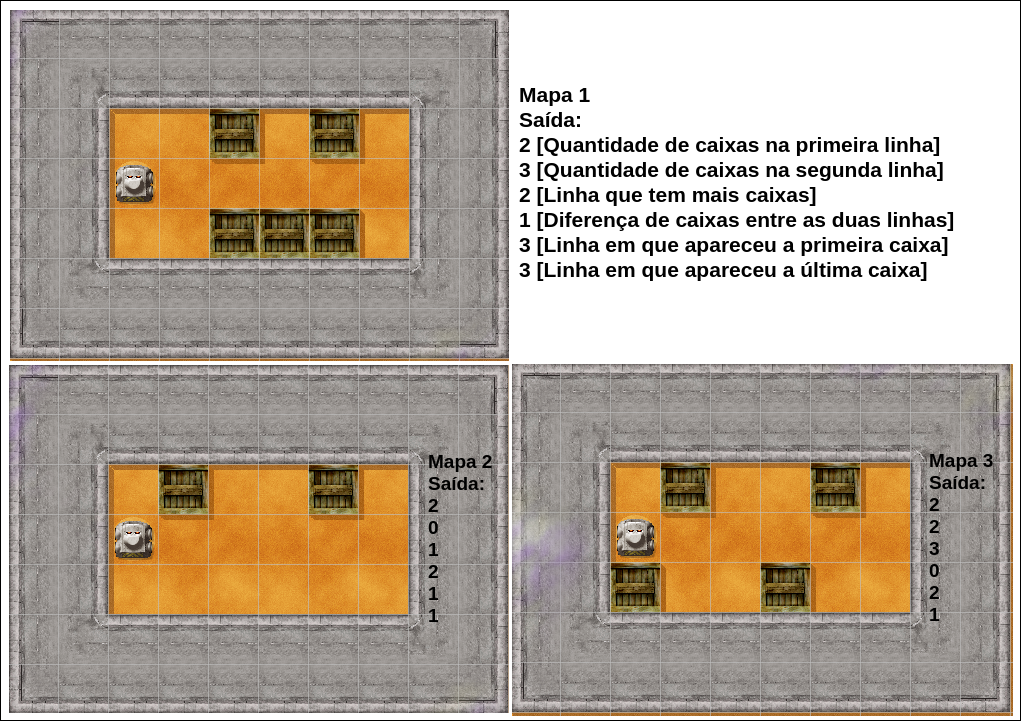
\includegraphics[height=10cm]{figuras/problema.png}
\fonte{\cite{furb}}
\label{fig:problem}
\end{figure}

Definido o problema, como próximo passo foi desenvolver uma solução para esse problema. Então desenvolvemos um programa ROBO capaz de apresentar as mesmas saídas para cada um desses mapas. A solução que propusemos contém cinco procedimentos e algumas variáveis que são suficientes para resolver o problema em questão. Na Figura \ref{fig:solution} tem um trecho do código ROBO proposto. Podemos notar que há uma estrutura de repetição (\texttt{repeatWhile}) com uma condição (\texttt{frontIsClear}) que verifica se a célula posterior ao robô está livre. Os cinco procedimentos definidos são: (1) \texttt{countLeft}, conta a quantidade de caixas à esquerda do robô; (2) \texttt{countRight}, conta a quantidade de caixas à direita do robô; (3) \texttt{showsMoreBoxes}, mostra qual linha tem mais caixas e a diferença entre elas; (4) \texttt{getBoxsFirstLine}, mostra a quantidade de caixas na primeira linha; por fim, (5) \texttt{getBoxLastLine}, mostra a quantidade de caixas na última linha.

\begin{figure}[h]
\centering
\caption{Solução proposta para o problema Contando Caixas}
\lstinputlisting[language=Java]{codes/solution.rob}
\fonte{O autor}
\label{fig:solution}
\end{figure}

Para validar a efetividade do compilador em integração com FDR, foi necessário verificar as saídas geradas pelo prótotipo e executar os traces gerados no ambiente RoboMind e as saídas geradas pelo FDR, além disso o FDR provê se a solução está livre de \textit{deadlock}, uma propriedade que o RoboMind não verifica. Na próxima seção estão os resultados obtido em ambas ferramentas.

\subsection{Resultados gerados}
\label{sub:sec43}

\begin{table}[]
\caption{Resultado obtido após a verificação do FDR}
\resizebox{\textwidth}{!}{%
\begin{tabular}{*{14}{|c}|}
\multicolumn{1}{c}{Map 1} & \multicolumn{1}{c}{Map 2} & \multicolumn{1}{c}{Map 3} \\
assert PROGRAM :{[}deadlock free {[}F{]}{]} & assert PROGRAM :{[}deadlock free {[}F{]}{]} & assert PROGRAM :{[}deadlock free {[}F{]}{]} \\
Result: Failed & Result: Failed & Result: Failed \\
Counterexample - Traces: & Counterexample - Traces: & Counterexample - Traces: \\
right() & right() & right() \\
forward(1) & forward(1) & forward(1) \\
forward(1) & forward(1) & forward(1) \\
forward(1) & forward(1) & forward(1) \\
forward(1) & forward(1) & forward(1) \\
forward(1) & forward(1) & forward(1) \\
show(2) & show(2) & show(2) \\
show(3) & show(0) & show(2) \\
show(2) & show(1) & show(3) \\
show(1) & show(2) & show(0) \\
show(3) & show(1) & show(2) \\
show(3) & show(1) & show(1)
\end{tabular}%
}
\fonte{O autor}
\end{table}

\subsection{Análise dos resultados}
\label{sub:sec44}
Levando-se em conta o que foi observado, para os três mapas analisados, comparando as saídas geradas pelo RoboMind e pela ferramenta proposta, é notório que a tradução dos programas foram realizadas corretamente, isto é, os programas CSP são semanticamente equivalentes a ROBO.


